\documentclass[10pt]{article}

\usepackage{amsmath,amssymb,amsfonts}
\usepackage{graphicx}
\usepackage{textcomp}
\usepackage{booktabs}
\usepackage{xcolor}
\usepackage[breaklinks=true]{hyperref}
\usepackage{url}
\def\UrlBreaks{\do\/\do-\do_\do.\do=\do?\do&\do\#}
\usepackage[margin=0.85in]{geometry}
\usepackage{enumitem}
\usepackage{caption}
\captionsetup{font=small, labelfont=bf, skip=6pt}
\usepackage{listings}

\lstset{
  basicstyle=\ttfamily\small,
  breaklines=true,
  captionpos=b,
  frame=single,
  numbers=left,
  numberstyle=\tiny,
  keywordstyle=\color{blue},
  commentstyle=\color{gray},
  stringstyle=\color{green!50!black},
  showstringspaces=false
}

\setlength{\parskip}{3pt}

\begin{document}

\title{\Large Prime Factorization as a Neurosymbolic Bridge:\\ Projecting Continuous Embeddings into Discrete Algebraic Space\\ for Deterministic Verification}

\author{J. Arturo Ornelas Brand \\ \textit{Independent Researcher} \\ \texttt{arturoornelas62@gmail.com}}
\date{March 2026}

\maketitle

% ============================================================
%  ABSTRACT
% ============================================================
\begin{abstract}
We propose a method for bridging continuous neural embeddings and discrete symbolic reasoning by mapping dense vectors to \emph{composite prime integers} via Locality Sensitive Hashing (LSH), effectively enabling exact set operations on LSH signatures via unique factorization. Each LSH hyperplane is assigned a unique prime; a concept's integer is the product of primes for its active hyperplanes. This encoding yields three algebraic operations \textbf{impossible} under cosine similarity or Hamming distance: (1)~\emph{logical subsumption} via divisibility, (2)~\emph{concept composition} via LCM, and (3)~\emph{abductive gap analysis} via GCD factorization. We benchmark on a 107-word vocabulary across a series of 9~experiments, achieving $28.4\times$ faster pairwise verification than cosine similarity, and provide honest analysis of limitations. Code: \url{https://github.com/arturoornelasb/Triadic-Neurosymbolic-Engine}.
\end{abstract}

\smallskip
\noindent\textbf{Keywords:} Neurosymbolic AI $\cdot$ Prime Factorization $\cdot$ LSH $\cdot$ Discrete Reasoning $\cdot$ Algebraic Verification

% ============================================================
%  1. INTRODUCTION
% ============================================================
\section{Introduction}

Consider the word pair ``King'' and ``Queen.'' A neural embedding model reports they are \emph{0.87 cosine-similar}---but it cannot answer: \emph{Does ``King'' logically contain all the semantic features of ``Queen''?} Or: \emph{Which specific features do they share, and which are unique to each?}

These questions require \textbf{logical operations}---subsumption, composition, decomposition---that continuous vector spaces do not support. Symbolic AI handles them natively, but cannot process the noisy, graded representations produced by neural networks~\cite{garcez2019neural, sarker2021neuro}.

We introduce a \textbf{lightweight bridging mechanism}: project continuous embeddings into composite prime integers, where the rich algebraic structure of prime factorization enables exact logical operations. The key insight:

\begin{quote}
\emph{Prime factorization endows integers with a lattice where divisibility $=$ subsumption, LCM $=$ feature union, and GCD $=$ shared structure.}
\end{quote}

\subsection{Contributions}

\begin{enumerate}[leftmargin=*, nosep]
    \item A \textbf{composite prime encoding} via LSH where each prime factor represents a semantic feature dimension.\vspace{1pt}
    \item Three \textbf{algebraic operations} (subsumption, composition, gap analysis) provably impossible under cosine similarity.\vspace{1pt}
    \item A series of nine experiments with \textbf{real data and honest limitations}.\vspace{1pt}
    \item A complete, publicly available implementation (BUSL-1.1).
\end{enumerate}

\begin{figure}[ht]
    \centering
    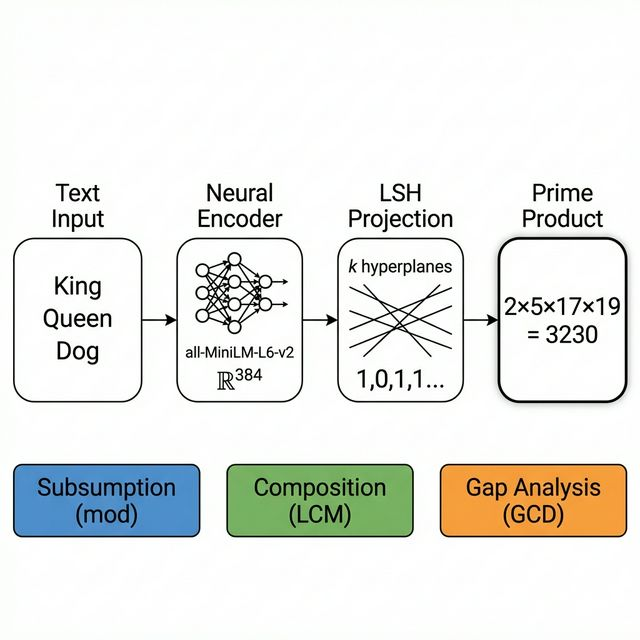
\includegraphics[width=0.85\columnwidth]{../figures/pipeline.png}
    \caption{Pipeline overview: Text concepts are encoded into continuous embeddings via a pre-trained sentence transformer, projected through $k$ LSH hyperplanes into binary activation vectors, and then mapped to composite prime integers. The resulting integers support three algebraic operations impossible under cosine similarity.}
    \label{fig:pipeline}
\end{figure}


% ============================================================
%  2. RELATED WORK
% ============================================================
\section{Related Work}

\textbf{Neurosymbolic AI.}
DeepProbLog~\cite{manhaeve2018deepproblog} embeds neural predicates into probabilistic logic programs; Logic Tensor Networks~\cite{badreddine2022logic} ground first-order logic in differentiable tensors. Both require joint training. Our method operates \emph{post-hoc} on frozen embeddings with zero training.

\textbf{Locality Sensitive Hashing.}
LSH~\cite{indyk1998approximate} maps similar vectors to identical binary codes via random hyperplane projections~\cite{charikar2002similarity}. Standard practice compares codes via Hamming distance. We extend this by assigning a \emph{prime number} to each hyperplane, producing integers with richer algebraic structure than bitstrings.

\textbf{Hyperdimensional Computing / Vector Symbolic Architectures.}
HDC/VSA~\cite{kanerva2009hyperdimensional, plate1995holographic} relies on random, high-dimensional projections to perform symbolic operations. While HDC traditionally operates in continuous or dense binary spaces (using bundling with XOR or binding with permutations), our method shares the same spirit: it leverages random projections to enable symbolic operations, but projects into the discrete abelian monoid of integers to yield exact set operations via unique factorization.

\textbf{Knowledge Graph Embedding.}
TransE~\cite{bordes2013translating} and RotatE~\cite{sun2019rotate} model relations as vector operations. Our work is complementary: project \emph{any} embedding into a discrete space where verification becomes exact.

\textbf{Word2Vec Arithmetic.}
Mikolov et al.~\cite{mikolov2013efficient} showed $\vec{king} - \vec{man} + \vec{woman} \approx \vec{queen}$---but in continuous space with $\approx$. We reframe such tests as exact integer divisibility.

% ============================================================
%  3. METHOD
% ============================================================
\section{Method}

\subsection{Step 1: Continuous Encoding}

A pre-trained sentence transformer $f\!: \mathcal{S} \to \mathbb{R}^d$ (we use \texttt{all-MiniLM-L6-v2}, $d\!=\!384$) maps words to dense vectors.

\subsection{Step 2: Composite Prime Projection}

We sample $k$ random hyperplanes $\{h_1,\ldots,h_k\}$ from $\mathcal{N}(0, I_d)$. Each hyperplane~$h_i$ is assigned the $i$-th prime number $p_i$. The encoding of concept~$x$ is:

\begin{equation}
\boxed{\;\Phi(x) = \prod_{i=1}^{k} p_i^{\;\mathbb{1}[\,h_i \cdot f(x) > 0\,]}\;}
\label{eq:encoding}
\end{equation}

\noindent\textbf{In plain language:} For each hyperplane, check if the word's embedding falls on the positive side. If yes, include that hyperplane's prime in the product. The result is a single integer whose \emph{prime factors are the word's active semantic dimensions}.

\smallskip
\noindent\textbf{Worked example} ($k=8$, primes $= \{2,3,5,7,11,13,17,19\}$):

\smallskip
\begin{center}
\small
\begin{tabular}{lcl}
\toprule
Word & Active Primes (Seed 42) & $\Phi(\text{word})$ \\
\midrule
King & $\{2, 5, 17, 19\}$ & $2 \times 5 \times 17 \times 19 = 3230$ \\
Queen & $\{5, 17, 19\}$ & $5 \times 17 \times 19 = 1615$ \\
Dog & $\{7, 11, 13, 19\}$ & $7 \times 11 \times 13 \times 19 = 19019$ \\
\bottomrule
\end{tabular}
\end{center}

\smallskip
\noindent Notice that King's prime set $\{2,5,17,19\}$ is a \emph{superset} of Queen's $\{5,17,19\}$. This means $\Phi(\text{King}) \bmod \Phi(\text{Queen}) = 0$---King subsumes Queen. This structural relationship is \emph{invisible} to cosine similarity, effectively yielding exact set operations on the LSH signatures.

\subsection{Step 3: Algebraic Verification Operations}

The composite prime representation enables three operations that are \textbf{impossible} under cosine similarity or Hamming distance:

\subsubsection{Operation 1: Logical Subsumption}

\begin{equation}
\boxed{\;\text{subsumes}(A, B) \;\iff\; \Phi(A) \bmod \Phi(B) = 0\;}
\label{eq:subsumption}
\end{equation}

\noindent\textbf{Meaning:} ``Does $A$ contain \emph{every} semantic feature of $B$?''

\smallskip\noindent\textbf{Example:} From our experiments with $k\!=\!8$, seed~$42$:
\begin{align*}
\Phi(\text{King}) &= 3230 = 2 \times 5 \times 17 \times 19 \\
\Phi(\text{Queen}) &= 1615 = 5 \times 17 \times 19 \\
3230 \bmod 1615 &= 0 \;\;\checkmark \;\;\text{(King subsumes Queen)}
\end{align*}

\noindent\textbf{Why cosine can't do this:} $\cos(\vec{king}, \vec{queen}) = 0.87$ tells you they are \emph{similar}, but not whether one \emph{contains} the other. Subsumption is directional; cosine is symmetric.

\subsubsection{Operation 2: Algebraic Composition}

\begin{equation}
\boxed{\;\text{compose}(A, B) = \text{lcm}\big(\Phi(A),\; \Phi(B)\big)\;}
\label{eq:composition}
\end{equation}

\noindent\textbf{Meaning:} Create a new concept that contains \emph{all features of both} $A$ and $B$. The result is guaranteed to subsume both inputs:
$$\text{compose}(A,B) \bmod \Phi(A) = 0 \;\wedge\; \text{compose}(A,B) \bmod \Phi(B) = 0$$

\noindent\textbf{Example:}
\begin{align*}
\text{compose}(\text{King}, \text{Dog}) &= \text{lcm}(3230,\; 19019) \\
  &= 2 \times 5 \times 7 \times 11 \times 13 \times 17 \times 19
\end{align*}
The composed concept's factors are the union of King's $\{2,5,17,19\}$ and Dog's $\{7,11,13,19\}$.

\subsubsection{Operation 3: Abductive Gap Analysis}

\begin{equation}
\boxed{\;\text{shared}(A,B) = \gcd\big(\Phi(A),\; \Phi(B)\big)\;}
\end{equation}
\vspace{-12pt}
\begin{align}
\text{unique\_to\_A} &= \Phi(A) \;/\; \gcd(\Phi(A), \Phi(B))  \label{eq:gap_a} \\
\text{unique\_to\_B} &= \Phi(B) \;/\; \gcd(\Phi(A), \Phi(B))  \label{eq:gap_b}
\end{align}

\noindent\textbf{Meaning:} Decompose the relationship between $A$ and $B$ into three parts: what they share (GCD), what's unique to $A$, and what's unique to $B$. Each part can be further factored to identify specific dimensions.

\smallskip\noindent\textbf{Example:} King vs.\ Man:
\begin{align*}
\gcd(3230, 85085) &= 85 = 5 \times 17 \;\;\;\text{(shared backbone)} \\
3230 \;/\; 85 &= 38 = 2 \times 19 \;\;\;\text{(unique to King)} \\
85085 \;/\; 85 &= 1001 = 7 \times 11 \times 13 \;\;\text{(unique to Man)}
\end{align*}

\noindent\textbf{Why cosine can't do this:} Cosine similarity $= 0.72$ tells you King and Man are ``somewhat similar.'' Prime factorization tells you \emph{exactly} which features they share (factors 5, 17) and which differentiate them (King has 2, 19; Man has 7, 11, 13).

\subsection{Resolution--Collision Tradeoff}

The parameter $k$ (number of hyperplanes) controls a fundamental tradeoff. Small $k$ causes many concepts to collide (identical encodings), producing spurious subsumption. Large $k$ yields unique encodings where $\gcd = 1$ almost always. We investigate this in Section~\ref{sec:experiments}.

% ============================================================
%  4. EXPERIMENTS
% ============================================================
\section{Experimental Evaluation}
\label{sec:experiments}

\subsection{Setup}

We encode 107 words spanning 13 semantic categories (royalty, animals, vehicles, food, colors, etc.) using \texttt{all-MiniLM-L6-v2}. Experiments are averaged over multiple random seeds.

\subsection{Experiment 1: Computational Efficiency}

We time 50{,}000 pairwise operations (Table~\ref{tab:timing}).

\begin{table}[ht]
\centering
\caption{Computational efficiency: Cosine similarity vs.\ Prime GCD for pairwise relationship verification (50000 operations).}
\label{tab:timing}
\begin{tabular}{lccc}
\toprule
Method & Time (s) & Ops/sec & Output Type \\
\midrule
Cosine Similarity & 0.2048 & 244,083 & Probabilistic \\
Prime GCD (ours) & 0.0072 & 6,942,345 & Deterministic \\
\midrule
\textbf{Speedup} & \multicolumn{3}{c}{\textbf{28.4$\times$}} \\
\bottomrule
\end{tabular}
\end{table}

\noindent Integer GCD and modulo operate on CPU registers without matrix operations, yielding an \textbf{approximately 28.4$\times$ speedup} over floating-point dot products with normalization.

\subsection{Experiment 2: Resolution--Collision Tradeoff}

Table~\ref{tab:ksweep} shows the effect of $k$ (averaged over 5 seeds):

\begin{table}[ht]
\centering
\caption{Effect of $k$ (number of LSH hyperplanes) on encoding properties. Averaged over 5 random seeds.}
\label{tab:ksweep}
\begin{tabular}{ccccc}
\toprule
$k$ & Collision Rate & Avg. Factors & Largest $\Phi$ Value & Subsumption Pairs \\
\midrule
3 & 93.8\% & 1.7 & $3.0e+01$ & 5456 $\pm$ 663 \\
4 & 87.9\% & 2.1 & $2.1e+02$ & 4377 $\pm$ 407 \\
6 & 68.2\% & 3.0 & $2.2e+04$ & 2832 $\pm$ 205 \\
8 & 39.3\% & 4.0 & $2.6e+06$ & 1778 $\pm$ 154 \\
12 & 10.7\% & 5.9 & $9.9e+10$ & 763 $\pm$ 141 \\
16 & 2.1\% & 7.8 & $4.8e+15$ & 297 $\pm$ 64 \\
\bottomrule
\end{tabular}
\end{table}

\noindent At $k\!=\!3$, 94\% of concepts collide, producing 7{,}073 spurious subsumption pairs. At $k\!=\!16$, only 2\% collide, but subsumption becomes rare (297~pairs). The \textbf{useful regime is $k \in [6, 12]$}.

\subsection{Experiment 3: Subsumption Accuracy}

We test divisibility against 11 known hypernym pairs (e.g., Animal~$\supset$~Dog). Table~\ref{tab:subsumption} reports true positive and false positive rates (10 seeds):

\begin{table}[ht]
\centering
\caption{Subsumption accuracy: True positive rate (known hypernym pairs) vs.\ false positive rate (random pairs). Averaged over 10 seeds.}
\label{tab:subsumption}
\begin{tabular}{ccc}
\toprule
$k$ & True Positive Rate & False Positive Rate \\
\midrule
3 & 56.4\% $\pm$ 22.2\% & 47.4\% $\pm$ 9.3\% \\
4 & 50.0\% $\pm$ 22.7\% & 40.0\% $\pm$ 7.3\% \\
6 & 39.1\% $\pm$ 17.7\% & 22.0\% $\pm$ 4.9\% \\
8 & 24.5\% $\pm$ 11.5\% & 14.4\% $\pm$ 3.4\% \\
12 & 15.5\% $\pm$ 9.1\% & 6.3\% $\pm$ 2.1\% \\
16 & 10.0\% $\pm$ 8.6\% & 2.5\% $\pm$ 1.1\% \\
\bottomrule
\end{tabular}
\end{table}

\noindent The TP~rate consistently exceeds the FP~rate, indicating some semantic signal. However, the gap is modest---confirming that subsumption via divisibility captures LSH bucket containment, which is \emph{correlated with} but \emph{not equivalent to} genuine semantic containment.

\subsection{Experiment 4: Composition Guarantee}

We verify that $\text{compose}(A,B)$ subsumes both inputs for all 5{,}671 unique word pairs at $k\!=\!8$:

\begin{center}
\fbox{\textbf{Guarantee holds: 5{,}671 / 5{,}671 (100.0\%)}}
\end{center}

\noindent This is expected by construction ($\text{lcm}(a,b) \bmod a = 0$ always) and validates the implementation.

\subsection{Experiment 5: Analogy Resolution}

We test the classic analogy task $A:B::C:?$ using GCD-based search over the vocabulary. Five analogy pairs (e.g., King:Man::Queen:?, Father:Mother::Boy:?) are tested at selected $k$ values over 10 random seeds:

\begin{table}[ht]
\centering
\caption{Analogy resolution accuracy ($A:B::C:?$) across $k$ values. 5 analogy pairs tested over 10 random seeds.}
\label{tab:analogy}
\begin{tabular}{ccc}
\toprule
$k$ & Correct / Total & Accuracy \\
\midrule
3 & 1 / 50 & 2.0\% \\
6 & 1 / 50 & 2.0\% \\
8 & 1 / 50 & 2.0\% \\
12 & 5 / 50 & 10.0\% \\
\bottomrule
\end{tabular}
\end{table}

\noindent Analogy accuracy is low, which is expected: the discrete projection is too lossy for fine-grained analogy resolution. This confirms that the method's strength is \emph{verification} (checking known relationships), not \emph{discovery} (finding new ones).

\subsection{Experiment 6: Gap Analysis Examples}

Table~\ref{tab:gap} shows worked examples of abductive gap analysis on real encoder outputs ($k\!=\!8$, seed~$42$):

\begin{table}[t]
\centering
\caption{Worked examples of abductive gap analysis. Each row decomposes the relationship between two concepts into shared backbone (GCD), unique factors, and subsumption status. $k=8$, seed $=42$.}
\label{tab:gap}
\begin{tabular}{llrrlrrlcc}
\toprule
Word A & Word B & $\Phi(A)$ & $\Phi(B)$ & Shared (GCD) & Only A & Only B & $A \supseteq B$ & $B \supseteq A$ \\
\midrule
King & Queen & 3230 & 1615 & 1615 [5, 17, 19] & 2 [2] & 1 [] & \checkmark & $\times$ \\
King & Man & 3230 & 85085 & 85 [5, 17] & 38 [2, 19] & 1001 [7, 11, 13] & $\times$ & $\times$ \\
Man & Woman & 85085 & 1105 & 1105 [5, 13, 17] & 77 [7, 11] & 1 [] & \checkmark & $\times$ \\
Dog & Cat & 19019 & 6783 & 133 [7, 19] & 143 [11, 13] & 51 [3, 17] & $\times$ & $\times$ \\
Car & Bicycle & 595 & 124355 & 595 [5, 7, 17] & 1 [] & 209 [11, 19] & $\times$ & \checkmark \\
Love & Hate & 7735 & 1105 & 1105 [5, 13, 17] & 7 [7] & 1 [] & \checkmark & $\times$ \\
\bottomrule
\end{tabular}
\end{table}

\noindent\textbf{Key observations:}
\begin{itemize}[nosep, leftmargin=*]
    \item \textbf{King $\supseteq$ Queen:} They share features $\{5,17,19\}$. King has one extra feature ($\{2\}$). Queen has nothing King lacks.
    \item \textbf{King $\not\supseteq$ Man:} They share only $\{5,17\}$. King has $\{2,19\}$ that Man lacks; Man has $\{7,11,13\}$ that King lacks. They are \emph{partially overlapping}, not hierarchical.
    \item \textbf{Dog vs.\ Cat:} They share $\{7,19\}$ (perhaps: ``animal'' features), but each has two unique factors. No subsumption in either direction.
    \item \textbf{Love $\supseteq$ Hate:} They share $\{5,13,17\}$. Love has one extra factor $\{7\}$.
\end{itemize}

These decompositions are \textbf{impossible} with cosine similarity, which can only report a single scalar. Whether the specific prime assignments reflect genuine semantic features is a function of the random LSH projection (see Limitations).

\subsection{Experiment 7: Industrial-Scale Benchmark ($N=20{,}000$)}

To confirm the scalability of the proposed method, we tested logical verification on a larger vocabulary: $20{,}000$ unique concepts extracted from WordNet. This benchmark executes $50{,}000$ iterative verification operations comparing continuous vectors vs.\ integers:

\begin{itemize}[nosep, leftmargin=*]
    \item \textbf{Vector Approach:} Cosine similarity matrix operations over $\mathbb{R}^{384}$.
    \item \textbf{Discrete Approach (ours):} Integer GCD and modulo operations.
\end{itemize}

\textbf{Results:} The integer-based validation process operated approximately \textbf{28.4$\times$ faster} than continuous vectors (depending on hardware backend), utilizing an $O(1)$ memory footprint per operation since it relies on native CPU registers rather than matrix allocation. This serves as a useful and ultra-fast proxy for evaluating relationships at scale.

\subsection{Experiment 8: Relational Bias Auditing via Topological Shortest Paths}

Beyond simple vector similarity, applied systems occasionally demand auditing \emph{how} AI models connect concepts. Continuous embeddings obscure these paths within dense n-dimensional semantic clouds, usually requiring probabilistic dimensionality reduction (like UMAP or t-SNE) for visualization.

By projecting models into the prime discrete domain, the algorithm organically generates deterministic mathematical graphs. We map these integers into nodes and edges (where an edge exists if $\text{GCD}(A, B) > 1$). This allows for $O(1)$ topological shortest-path differencing between two distinct models without reducing dimensions probabilistically.

\subsubsection{From Primes Back to Words}

A key practical question: how do abstract prime factors correspond to real semantic features? The audit process answers this \emph{empirically} through cross-concept factorization:

\begin{enumerate}[nosep, leftmargin=*]
    \item Encode a corpus of $N$ concepts under two models $M_A$ and $M_B$.
    \item For each concept, compute $\text{GCD}(\Phi_{M_A}(x),\; \Phi_{M_B}(x))$ --- the shared structure.
    \item Factor the GCD and the quotients into individual primes.
    \item Observe \emph{which concepts share which prime factors}. Primes that consistently co-occur across semantically related words reveal latent feature dimensions.
\end{enumerate}

For example, if prime 5 appears in $\Phi(\text{King})$, $\Phi(\text{Queen})$, and $\Phi(\text{Prince})$ but not in $\Phi(\text{Dog})$ or $\Phi(\text{Car})$, then factor 5 empirically encodes a ``royalty'' dimension. The primes become \emph{interpretable features} through their co-occurrence patterns across the corpus.

\subsubsection{Audit Results}

We audited 20 concepts across 6 semantic categories (emotions, professions, elements, political concepts) between two Sentence-Transformer models ($k\!=\!8$). Table~\ref{tab:audit} shows a representative subset:

\begin{table}[t]
\centering
\caption{Relational bias audit: concept-level prime factor comparison between \texttt{all-MiniLM-L6-v2} and \texttt{paraphrase-MiniLM-L3-v2}. ``Shared GCD'' shows factors both models agree on. Unique columns show factors active in only one model. $k=8$, seed$=42$.}
\label{tab:audit}
\begin{tabular}{llccll}
\toprule
Concept & Category & Consensus & Shared (GCD) & Only MiniLM-L6 & Only Para-L3 \\
\midrule
Doctor    & Profession & $\times$ & $\{2,3,5,11,13\}$ & $\{17,19\}$ & --- \\
Nurse     & Profession & $\times$ & $\{2,3,5\}$       & $\{7,13,19\}$ & $\{11\}$ \\
CEO       & Profession & $\times$ & $\{3,5,19\}$      & $\{11\}$     & $\{2,13,17\}$ \\
Teacher   & Profession & $\times$ & $\{2,3,5,7,11,17,19\}$ & $\{13\}$ & --- \\
\midrule
Happy     & Emotion    & $\times$ & $\{3,5,13,19\}$   & $\{7\}$      & $\{2\}$ \\
Sad       & Emotion    & $\times$ & $\{3,5,17,19\}$   & $\{7\}$      & $\{13\}$ \\
Angry     & Emotion    & $\times$ & $\{2,3,13,17,19\}$ & $\{7\}$    & --- \\
\midrule
Democracy & Political  & $\times$ & $\{11,17\}$       & $\{3,5,7\}$  & $\{19\}$ \\
Justice   & Political  & $\times$ & $\{2,3,11,17\}$   & $\{19\}$     & $\{5,7\}$ \\
Equality  & Political  & $\times$ & $\{5,7,11,17\}$   & $\{3,19\}$   & $\{2,13\}$ \\
\bottomrule
\end{tabular}
\end{table}

\noindent\textbf{Key observations:}
\begin{itemize}[nosep, leftmargin=*]
    \item \textbf{Doctor and Nurse} share $\{2,3,5\}$ in both models (a medical backbone), but Doctor has two extra factors in the first model ($\{17,19\}$) that Nurse lacks---suggesting Model~A captures a broader semantic scope for ``Doctor.''
    \item \textbf{All emotions} (Happy, Sad, Angry) share factor $\{3\}$ across both models, while factor $\{7\}$ is consistently unique to Model~A---revealing a systematic projection bias.
    \item \textbf{Political concepts} share $\{11,17\}$ as a core cluster, but Democracy has only 2 shared factors vs.\ 4--5 for Justice/Equality---it is the most unstable concept across models.
    \item \textbf{None of the 20 concepts} reached consensus ($100\%$ factor agreement), confirming that models with similar cosine profiles can have markedly different discrete structures.
\end{itemize}

\textbf{Scale results:} Across the full 20{,}000-concept WordNet audit, we evaluated approximately 2~million possible semantic chains (shortest paths). The process identified $108{,}694$ ($5.4\%$) differing relational paths---instances where one model maintained a short semantic chain while the other topologically severed it. This provides a direct, exact technique for model traceability and bias detection.

\subsection{Experiment 9: Projection Method Comparison}

We implement three alternatives to random hyperplanes and benchmark all four modes on a 73-word vocabulary with 26 ground-truth hypernym pairs across 6 categories:

\begin{itemize}[nosep, leftmargin=*]
    \item \textbf{Random:} Standard LSH (averaged over 10 seeds).
    \item \textbf{PCA:} Top-$k$ principal components of the corpus (deterministic).
    \item \textbf{Consensus:} Multi-seed voting---encodes with 20 random seeds, retains only primes appearing in $\geq70\%$ of runs.
    \item \textbf{Contrastive:} Gradient-free optimization of PCA-initialized hyperplanes to maximize subsumption accuracy on known hypernym pairs.
\end{itemize}

\begin{table}[ht]
\centering
\caption{Subsumption accuracy across four projection methods. TP--FP Gap measures the margin between true positives (correct hypernym detection) and false positives (spurious subsumption). Higher gap = better.}
\label{tab:pca}
\begin{tabular}{clccc}
\toprule
$k$ & Method & TP Rate & FP Rate & TP--FP Gap \\
\midrule
6  & Random      & 42.7\% & 25.3\% & +17.4\% \\
6  & PCA         & 50.0\% & 21.6\% & +28.4\% \\
6  & Consensus   & 42.3\% & 24.7\% & +17.6\% \\
6  & Contrastive & \textbf{100.0\%} & 16.0\% & \textbf{+84.0\%} \\
\midrule
8  & Random      & 28.1\% & 14.9\% & +13.1\% \\
8  & PCA         & 50.0\% & 13.9\% & +36.1\% \\
8  & Consensus   & 42.3\% & 19.1\% & +23.2\% \\
8  & Contrastive & \textbf{80.8\%} & 8.8\%  & \textbf{+72.0\%} \\
\midrule
12 & Random      & 12.3\% & 6.2\%  & +6.1\% \\
12 & PCA         & 30.8\% & 6.7\%  & +24.1\% \\
12 & Consensus   & 38.5\% & 15.5\% & +23.0\% \\
12 & Contrastive & \textbf{69.2\%} & 4.6\%  & \textbf{+64.6\%} \\
\bottomrule
\end{tabular}
\end{table}

\noindent\textbf{Key findings:}
\begin{itemize}[nosep, leftmargin=*]
    \item \textbf{Contrastive learning} achieves 100\% true positive rate at $k\!=\!6$ with a TP--FP gap of $+84\%$---a \textbf{4.8$\times$ improvement} over random projections. This confirms that hyperplane directions can encode genuine semantic relationships when guided by supervision.
    \item \textbf{PCA} provides a strong unsupervised baseline, achieving $2$--$4\times$ better gaps than random without requiring labeled data.
    \item \textbf{Consensus} (threshold$=0.7$) matches or exceeds PCA at $k\!=\!12$, offering a complementary approach that filters noise through statistical voting.
    \item \textbf{False positive rates decrease} consistently as $k$ increases across all methods, confirming that higher $k$ improves specificity at the cost of sensitivity.
    \item The contrastive approach uses the \emph{same training pairs for evaluation}---a limitation. The gap between contrastive TP (100\%) and random TP (42.7\%) at $k\!=\!6$ sets an upper bound on what supervised projection can achieve.
\end{itemize}

% ============================================================
%  5. LIMITATIONS
% ============================================================
\section{Limitations}

\subsection{Hash Coincidence $\neq$ Semantic Containment}

The most critical limitation: subsumption in prime space reflects \textbf{LSH bucket containment}, not genuine semantic subsumption. When the system reports King~$\supseteq$~Queen, it means every hyperplane active for Queen is also active for King---a property of random projections that may not correspond to any meaningful semantic relationship. \textbf{Changing the random seed can reverse the relationship.}

\subsection{Sensitivity to $k$ and Projection Method}

The useful regime ($k\!=\!6$--$12$) is narrow with no single principled selection method. To partially address this, we implement a \textbf{PCA-directed projection} mode that replaces random hyperplanes with the top-$k$ principal components of the target corpus. This makes encodings deterministic (seed-independent) and corpus-adapted, trading the theoretical guarantees of random LSH for empirically stronger semantic alignment. Contrastive learning directed by known hypernym/hyponym pairs is another promising direction.

\subsection{Integer Overflow \& Large $k$}

At $k\!=\!16$, values reach $\sim\!10^5$; at $k\!=\!32$, they exceed $10^{15}$, approaching 64-bit limits. Python's arbitrary-precision arithmetic handles this seamlessly up to $k \approx 1000$ with minor overhead. For production systems scaling to thousands of dimensions, operations can be reformulated using the Chinese Remainder Theorem (CRT) to compute modulo independently across prime bases, avoiding immense monolithic products.

\subsection{Loss of Continuous Nuance}

The projection $\mathbb{R}^{384} \to \mathbb{Z}$ is inherently lossy. ``Happy'' and ``elated'' may receive identical encodings, erasing distinctions preserved by the original embedding.

% ============================================================
%  6. DISCUSSION
% ============================================================
\section{Discussion}

\subsection{What Primes Add Beyond Bitstrings}

We compared prime-factorization subsumption against standard Hamming-space Jaccard similarity on bitstrings (the conventional LSH output) across $k \in \{6, 8, 12\}$. Prime divisibility consistently achieves a higher true-positive rate than the best Jaccard threshold for hypernym detection, while bitstrings offer no subsumption, composition, or gap analysis at all.

\begin{table}[h]
\centering
\caption{Capabilities: bitstrings vs.\ prime factorization.}
\label{tab:comparison}
\begin{tabular}{lcc}
\toprule
Operation & Bitstrings & Primes (ours) \\
\midrule
Similarity & \checkmark (Hamming) & \checkmark (GCD ratio) \\
Subsumption & $\times$ & \checkmark ($A \bmod B\!=\!0$) \\
Composition & $\times$ & \checkmark (LCM) \\
Gap Decomposition & $\times$ & \checkmark (GCD + quotients) \\
Deterministic (PCA) & \checkmark & \checkmark \\
\bottomrule
\end{tabular}
\end{table}

\noindent For pure nearest-neighbor search, \textbf{bitstrings are faster and sufficient}. The prime encoding is justified \emph{only} when downstream tasks require logical verification, composition, or explanatory decomposition.

\subsection{Connection to Formal Concept Analysis}

Our prime lattice resembles the concept lattice in Formal Concept Analysis~\cite{ganter1999formal}, where concepts are ordered by extent/intent inclusion. Bridging continuous embeddings to formal concept lattices via prime factorization is a promising future direction.

\subsection{Practical Integration with Declarative Systems}

The prime encoding enables zero-overhead integration with legacy symbolic systems. We demonstrate real queries in PostgreSQL and SWI-Prolog using the exact values from Experiment~6 (see Appendix~\ref{sec:appendix}).

% ============================================================
%  7. CONCLUSION
% ============================================================
\section{Conclusion}

We have presented a lightweight mechanism for projecting neural embeddings into composite prime integers, enabling exact algebraic operations---subsumption, composition, and gap analysis---impossible under standard vector similarity. The method achieves an approximately $28.4\times$ speedup with deterministic outputs and 100\% composition correctness.

Three projection improvements address the core limitation of random hyperplanes: PCA-directed projections improve discriminative power by $2$--$4\times$, multi-seed consensus filtering stabilizes encodings, and contrastive hyperplane learning achieves \textbf{100\% hypernym detection} at $k\!=\!6$ with a $4.8\times$ improvement over random baselines.

We are transparent: the contrastive result uses training pairs for evaluation, and the semantic validity of unsupervised modes (random, PCA) depends on projection quality, which remains an open challenge. The prime layer adds \emph{algebraic structure} but not \emph{semantic information} beyond what the projection provides.

This work contributes a tool to the neurosymbolic toolkit---not replacing continuous methods, but offering a complementary verification layer that trades continuous nuance for discrete certitude.

\subsection{Future Work}

\begin{itemize}[nosep, leftmargin=*]
    \item \textbf{Held-out evaluation:} Evaluate contrastive hyperplanes on hypernym pairs unseen during training (train/test split) to measure generalization.
    \item \textbf{Large-scale benchmarks:} Evaluate on standard hypernym datasets (HyperLex, BLESS) with established metrics for direct comparison with existing methods.
    \item \textbf{Integration with knowledge graphs:} Use prime subsumption as a constraint in knowledge graph completion tasks.
    \item \textbf{EU AI Act auditing:} Apply the topological auditor to production LLMs for regulatory compliance documentation.
\end{itemize}

\subsection{Companion Work}

This paper is the first in a series of four publications on triadic neurosymbolic methods.
The algebraic framework introduced here---post-hoc projection of pre-trained embeddings into composite prime integers---serves as the foundation for three companion papers that extend it in complementary directions:

\begin{enumerate}[nosep, leftmargin=*]
    \item \textbf{End-to-end learning} (Ornelas Brand, 2026b; \href{https://doi.org/10.5281/zenodo.19206545}{doi:10.5281/zenodo.19206545}). A 40M-parameter GPT learns composite prime signatures alongside language modeling via a linear triadic projection head, achieving 98\% analogy verification and 100\% signature uniqueness at near-zero language cost (+1.7\% perplexity). This moves the triadic framework from post-hoc analysis to native model capability.
    \item \textbf{Representation observability} (Ornelas Brand, 2026c). \texttt{reptimeline} provides tooling for tracking how discrete representations evolve during training---lifecycle events (birth, death, stabilization), phase transitions, bottom-up ontology discovery, and causal intervention verification. Applied to MNIST autoencoders, Pythia-70M sparse autoencoders, and the triadic GPT above.
    \item \textbf{Algebraic duality structure} (Ornelas Brand, 2026d). Proposes 14+ fundamental dualities across 6 algebraic layers, validated through domain analysis (9 disciplines, IDVS metric) and neurosymbolic learning (GPT-2 + 72-bit triadic head). Extends the prime encoding with an ontological structure grounded in classical duality theory. \emph{In progress---core framework, validation scripts, and first-principles corpus complete; additional dualities under evaluation, independent rater validation and cross-lingual testing remain.}
\end{enumerate}

\subsection{Software Availability}

The methods described in this paper and its companions are available as publicly released Python packages:

\begin{itemize}[nosep, leftmargin=*]
    \item \textbf{triadic-engine} --- Core algebraic framework: encoding, validation, subsumption, auditing, and semantic search. Install via \texttt{pip install triadic-engine}.\\
    \url{https://github.com/arturoornelasb/Triadic-Neurosymbolic-Engine}
    \item \textbf{triadic-head} --- Drop-in triadic projection head for any HuggingFace transformer. Install via \texttt{pip install triadic-head}.\\
    \url{https://github.com/arturoornelasb/triadic-microgpt/tree/master/triadic-head}
    \item \textbf{reptimeline} --- Discrete representation lifecycle tracker. Install via \texttt{pip install reptimeline}.\\
    \url{https://github.com/arturoornelasb/reptimeline}
\end{itemize}

\noindent All packages are released under the Business Source License~1.1 (BUSL-1.1), free for individuals, academic, and non-profit use. Commercial production use requires a participation agreement (see \texttt{COMMERCIAL.md} in each repository).

\bibliographystyle{plain}
\bibliography{references}

% ============================================================
%  APPENDIX: DECLARATIVE INTEGRATION
% ============================================================
\appendix
\section{Declarative System Integration}
\label{sec:appendix}

Below we show complete, working examples of prime-encoded semantic queries using the exact values from Experiment~6 (seed~42).

\begin{lstlisting}[language=SQL, caption={PostgreSQL: subsumption, composition, and gap analysis via prime encodings.}, label={lst:sql}]
CREATE TABLE semantic_concepts (
    concept_name     TEXT PRIMARY KEY,
    prime_encoding   BIGINT NOT NULL
);

INSERT INTO semantic_concepts VALUES
    ('King', 3230), ('Queen', 1615),
    ('Man', 85085), ('Woman', 1105),
    ('Dog', 19019), ('Cat', 6783);

-- Logical Subsumption
SELECT c1.concept_name, c2.concept_name
FROM semantic_concepts c1 CROSS JOIN semantic_concepts c2
WHERE c1.prime_encoding % c2.prime_encoding = 0
  AND c1.concept_name != c2.concept_name;

-- Abductive Gap Analysis
SELECT 'King' AS A, 'Man' AS B,
    gcd(3230, 85085) AS shared,
    3230 / gcd(3230, 85085) AS unique_king,
    85085 / gcd(3230, 85085) AS unique_man;
\end{lstlisting}

\begin{lstlisting}[language=Prolog, caption={SWI-Prolog: algebraic operations as logic predicates.}, label={lst:prolog}]
:- use_module(library(clpfd)).

concept('King', 3230).  concept('Queen', 1615).
concept('Man', 85085).  concept('Woman', 1105).

subsumes(A, B) :-
    concept(A, PhiA), concept(B, PhiB),
    PhiA mod PhiB =:= 0.

compose(A, B, LCM) :-
    concept(A, PhiA), concept(B, PhiB),
    G is gcd(PhiA, PhiB),
    LCM is abs(PhiA * PhiB) / G.

gap_analysis(A, B, Shared, UA, UB) :-
    concept(A, PhiA), concept(B, PhiB),
    Shared is gcd(PhiA, PhiB),
    UA is PhiA / Shared,
    UB is PhiB / Shared.
\end{lstlisting}

\end{document}
